\documentclass[11pt, a4paper]{article}
\usepackage{graphicx, fullpage, hyperref, listings}
\usepackage{appendix, pdfpages, color}
\usepackage{indentfirst} %段首空两格 棒
\usepackage{chngpage} 
\usepackage{tocloft}            % This squashes the Table of Contents a bit
\usepackage{pdfpages}
\usepackage{multirow}
\usepackage{amsmath}
\usepackage{framed}


\setlength\cftbeforesecskip{3pt}
\renewcommand{\contentsname}{\centerline{\textbf{Content}}}
\graphicspath{{images/}}

\usepackage{multicol}

\usepackage{graphicx}
\usepackage{epstopdf}
\hypersetup{CJKbookmarks,%
	bookmarksnumbered,%
	colorlinks,%
	linkcolor=black,%
	citecolor=black,%
	plainpages=false,%
	pdfstartview=FitH}

%%%%%%%代码语法高亮设置

\usepackage{color}

\definecolor{pblue}{rgb}{0.13,0.13,1}
\definecolor{pgreen}{rgb}{0,0.5,0}
\definecolor{pred}{rgb}{0.9,0,0}
\definecolor{pgrey}{rgb}{0.46,0.45,0.48}

\usepackage{listings}
\lstset{
	language=Java,
	showspaces=false,
	showtabs=false,
	%%%%%
	frame = single,
	stepnumber = 2,  
	numbersep = 4pt, 
	numbers=left,
	%breakatwhitespace=false, 
	tabsize=2,  
	%%%%%
	breaklines=true,
	showstringspaces=false,
	breakatwhitespace=false, 
	commentstyle=\color{pgreen},
	keywordstyle=\color{pblue},
	stringstyle=\color{pred},
	basicstyle=\ttfamily,
	%moredelim=[il][\textcolor{pgrey}]{$$},
	%moredelim=[is][\textcolor{pgrey}]{\%\%}{\%\%},
}


%%%%%%%%代码语法高亮设置

\definecolor{MyLightYellow}{cmyk}{0,0.,0.2,0} 

\setlength{\parskip}{4pt}        % sets spacing between paragraphs
\interfootnotelinepenalty=500    % this prevents footnotes breaking across pages

\title{
\includegraphics[width=0.45\textwidth]{wpi2}
	\\CS 534 Artificial Intelligence \\ Assignment 4 }          % <<<<<<<<< change the title as appropriate
\author{Group 10 }                    % <<<<<<<<< module code

\begin{document}
	\begin{titlepage}
		
		%\date{\today}
		\maketitle
		\addtocontents{toc}{\protect\thispagestyle{empty}} % because we don't want a page number on the title page
		% Thanks to Huang Shanyue for suggesting this 
		
		\begin{center}
			Group Member
		\end{center}
		
		\begin{table}[htbp] 
			\begin{center}
				\begin{tabular}{l l l} 
					
					Yixuan & Jiao  &   yjiao@wpi.edu \\
					Yinkai & Ma  &   yma7@wpi.edu \\
					Jiaming & Nie  &  jnie@wpi.edu \\
					Pinyi & Xiao  &  pxiao@wpi.edu \\
				\end{tabular}
			\end{center}
		\end{table}
		
		
		
		%\date{\today}
		\thispagestyle{empty}  %去除首页页码
		
	\end{titlepage}

%\tableofcontents
%\listoffigures

%\newpage



\tableofcontents

%\listoffigures
%\listoftables
%\lstlistoflistings        


\newpage






\bibliographystyle{IEEEtran}  
%\bibliography{MyRefs} 
%\addcontentsline{toc}{section}{References}

\section{Program Description}

Our program is to solve a gridworld problem by creating an agent that uses reinforcement learning. In the gridworld, there are three special states: start, goal, pit (the goal and pit offer reward to the agent). For each movement, the agent will get a reward. The goal of agent in each trial is to gain most reward that it can. For each trial, we randomly pick a start state (any grid except goal and pits) and calculate its lookup table by using Q-function. And then use $\epsilon$-greedy to help the agent explore. The agent has five actions to choose for each step: up, down, left, right, and give up. There is a $\epsilon$ value of probability that the agent will choose a random action, and a $1-\epsilon$ value of probability that the agent will choose the action that has a maximum Q value. If the agent chose to give up, the trial will end and calculate total reward, otherwise we use actions that the agent chose with the corresponding Q values to update the old Q value of that initial step. However, because the uncertainty of the environment, there is 70$\%$ chance that the agent takes the expected movement, 10$\%$ chance it winds up at 90 degree right, 10$\%$ chance it winds up at 90 degree left, and 10$\%$ chance that it moves 2 squires forward. Then we repeat all of above steps from the grid that it winds up with until it gives up, gets in a pit, or reaches the goal. Finally, we calculate the total reward of the trial, and then restart for another trial. Through the whole process, the learned states of the gridworld are reserved for the following iterations, so that the agent can reinforce its learning and make better decision.


\section{Approach}

\subsection{Set up the gridworld and random start(not a goal or pit)}

\begin{itemize}
\item We store the state status in a dictionary by using “i * 10 + j” to represent the key of state coordination (i+1, j+1), for example, “key 35” means it is row 4, column 6. We memorize the Q-values of each normal grid state by storing the action values of each state in a “five numbers list” to represent the rewards of the state for moving "Up, Down, Left, Right, Give up". For pits and goal, we use “int” type to store the reward value.

\item Start with a randomly picked point (except goal and pits).

\end{itemize}

\subsection{Calculate Q-value lookup table by using SARSA and Roll dice to decide the actions}

\begin{itemize}
\item For each step, make action decision by generating a random P (range from 0 to 1), then compare P with $\epsilon$. If $P < \epsilon$, randomly pick an action and calculate the corresponding Q-value , otherwise, take the action that has the maximum Q-value, which is calculated by using $Q(s, a) = Q(s,a) + α(R(s) + \gamma Q(s’,a’) – Q(s,a))$, where $\gamma = 1$.

\item Use if statement to judge the state that next to the “Wall” in order to make sure the agent bounced back once it hits a wall.

\item At anytime, if the agent decide to give up or get into a pit or goal, the trial end. If the trial doesn’t end after the first action from the initial state, the agent will repeat “step 2.(1)” to see Q(s’,a’).

\end{itemize}

\subsection{Calculate new value and update}
\begin{itemize}
	\item Update the Q(s,a) by using the Q(s’,a’)
\end{itemize}


\subsection{Calculate the place it will wind up}

\begin{itemize}
	\item Generate a random P2 (range from 0 to 1). If $P2 > 0.3$, then the agent will take the movement as expected in step 2; if $P2 < 0.1$, it will go 90 degree left; if $0.1<= P2 <= 0.2$, it will go 90 degree right; $0.2 < P2 <= 0.3$, it will move forward 2 steps.
	
\end{itemize}

\subsection{Total Reward Calculation}

\begin{itemize}
\item Repeat from the second step until the trial end(goal, pit, or give up), and then calculate the total reward of the trial.
	
\item Total reward = number of steps * Movement Reward + State Reward/Give up Reward.
	
\end{itemize}

\subsection{Restart}

Restart another trial by using the environment that the agent learned from former trials.

\section{Write Up Questions Solution}


\subsection{Program Result Asymptote Plot}

In figure~\ref{fig:1_1}, the asymptote plot of scores vs. iterations is demonstrated. The number of iterations is 10000, take the median every 50 iterations and the parameters are on the following:

$\epsilon = 0.0$, $\alpha = 0.5$ 

\subsubsection{Iterations = 10000 Asymptote Plot} 

 \begin{figure}[htbp] 
	\begin{center}
		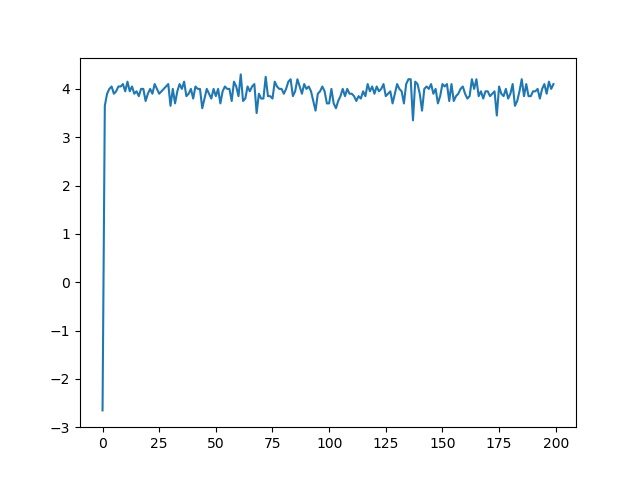
\includegraphics[width=8cm]{1_1W} 
		\caption{Scores vs. Iterations Model Training Result} 
		\label{fig:1_1}
		%插入图片的标题,一般放在图片的下方,放在表格的上方
	\end{center}
\end{figure}

\subsubsection{Iterations = 1000 Asymptote Plot}

The asymptote plot of scores vs. iterations is illustrated in figure~\ref{fig:1_2}, the parameters in this model are $\epsilon = 0.0$, $\alpha = 0.5$. 

 \begin{figure}[htbp] 
	\begin{center}
		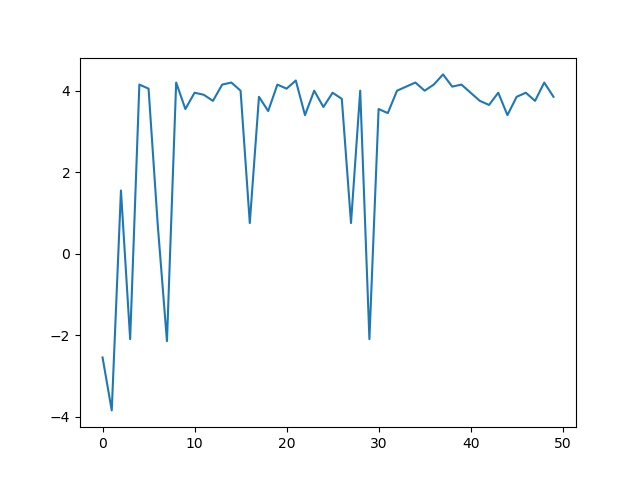
\includegraphics[width=8cm]{1_1K} 
		\caption{Scores vs. Iterations Model Training Result} 
		\label{fig:1_2}
		%插入图片的标题,一般放在图片的下方,放在表格的上方
	\end{center}
\end{figure}

\subsubsection{Map Movements}

The movements on the map is illustrated in figure~\ref{fig:1_3}, the symbols meanings are in the table~\ref{tab:movement}.

\begin{table}[htbp] 
	\begin{center}
		\caption{Movement Symbols}
		\begin{tabular}{c|l} \hline
		 Symbols & Meaning  \\ \hline
		 P     & Pit State \\ \hline
		 G    &  Goal State   \\ \hline
		 $\vee$  & Move Up  \\ \hline
		 $\wedge$  & Move Down \\ \hline
		 $<$  & Move Left  \\ \hline
		 $>$  & Move Right \\ \hline 
 			
		\end{tabular}
		\label{tab:movement}
	\end{center}
\end{table}	

%\newpage
The goal reward is 5, pit reward is -2, move reward is -0.1 and give up reward is -3.

 \begin{figure}[htbp] 
	\begin{center}
		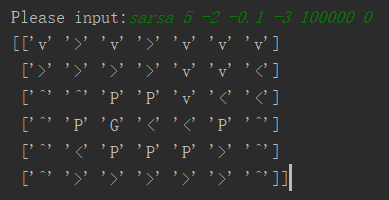
\includegraphics[width=6cm]{1_movement} 
		\caption{Movement Map} 
		\label{fig:1_3}
		%插入图片的标题,一般放在图片的下方,放在表格的上方
	\end{center}
\end{figure}

\newpage
The score map for each grid is on the following figure~\ref{fig:1_4}. 

\begin{figure}[htbp] 
	\begin{center}
		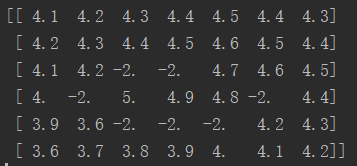
\includegraphics[width=4cm]{1_score} 
		\caption{Movement Map} 
		\label{fig:1_4}
		%插入图片的标题,一般放在图片的下方,放在表格的上方
	\end{center}
\end{figure}
 

\subsection{$\alpha$ Optimization}

In this part, different asymptotes plot will be compared to the $\alpha = 0.5$.

\subsubsection{$\alpha = 0.5$}

The asymptote plot of the $\alpha = 0.5$ is shown in figure~\ref{fig:2_2}. 

\begin{figure}[htbp] 
	\begin{center}
		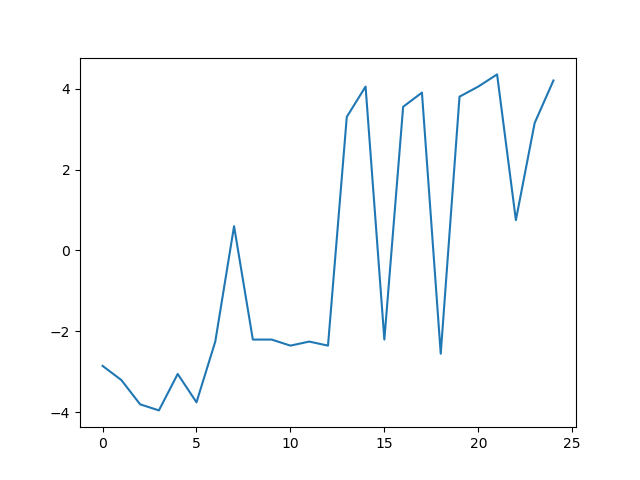
\includegraphics[width=6cm]{2_2} 
		\caption{$\alpha = 0.05$ Iterations = 1000} 
		\label{fig:2_2}
		%插入图片的标题,一般放在图片的下方,放在表格的上方
	\end{center}
\end{figure}


\subsubsection{$\alpha = 0.05$}

The asymptote plot of the $\alpha = 0.05$ is shown in figure~\ref{fig:2_1}

\begin{figure}[htbp] 
	\begin{center}
		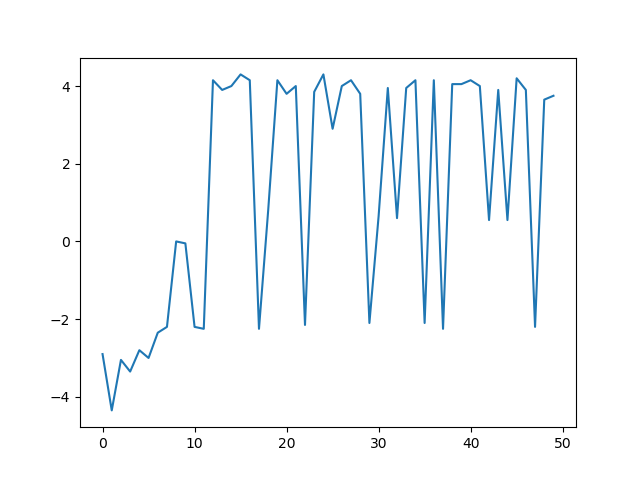
\includegraphics[width=6cm]{2_1} 
		\caption{$\alpha = 0.05$ Iterations = 1000} 
		\label{fig:2_1}
		%插入图片的标题,一般放在图片的下方,放在表格的上方
	\end{center}
\end{figure}


\subsubsection{$\alpha = 1$}

The asymptote plot of the $\alpha = 1$ is shown in figure~\ref{fig:2_3}

\begin{figure}[htbp] 
	\begin{center}
		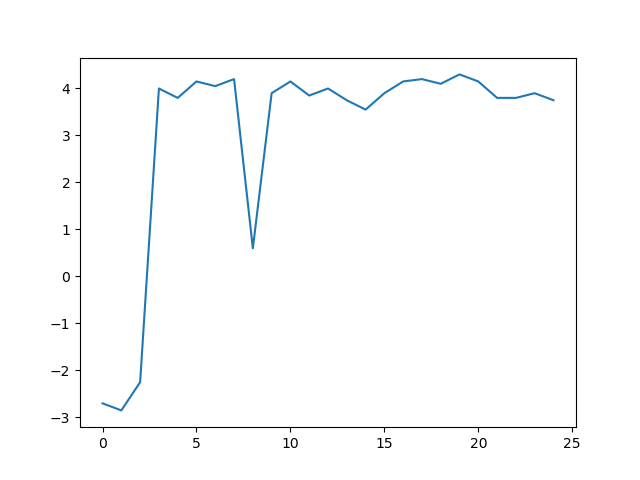
\includegraphics[width=7cm]{2_3} 
		\caption{$\alpha = 1$ Iterations = 1000} 
		\label{fig:2_3}
		%插入图片的标题,一般放在图片的下方,放在表格的上方
	\end{center}
\end{figure}


\subsection{$\epsilon = 0.2$ Asymptotes}

\subsubsection{Iterations = 1000}

In the figure~\ref{fig:3_1}, the result asymptote plot under the situation $\epsilon = 0.2$ is illustrated. Compared to figure~\ref{fig:1_2} with $\epsilon = 0$, the $\epsilon = 0.2$ illustrated the convergence result with slower result. 

\begin{figure}[htbp] 
	\begin{center}
		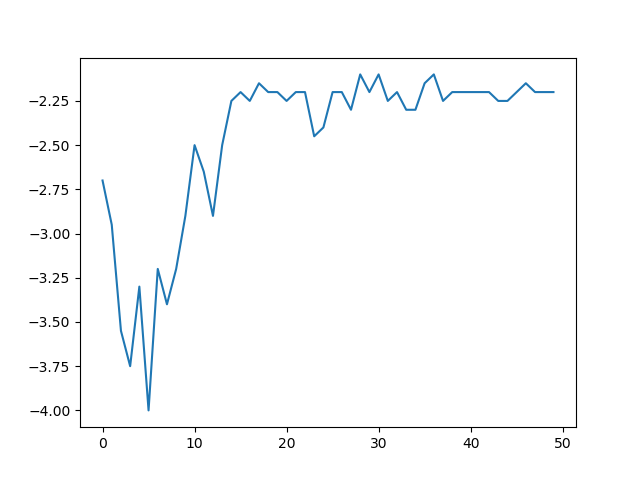
\includegraphics[width=7cm]{3_e_2} 
		\caption{$\epsilon = 0.2$ Asymptote Plot Iterations = 1000} 
		\label{fig:3_1}
		%插入图片的标题,一般放在图片的下方,放在表格的上方 
	\end{center}
\end{figure}

\subsubsection{Iterations = 10000}

In the figure~\ref{fig:3_2}, the result asymptote plot under the situation $\epsilon = 0.2$ is illustrated. Compared to figure~\ref{fig:1_2} with $\epsilon = 0$, the $\epsilon = 0.2$ illustrated the convergence result with slower result. 

\begin{figure}[htbp] 
	\begin{center}
		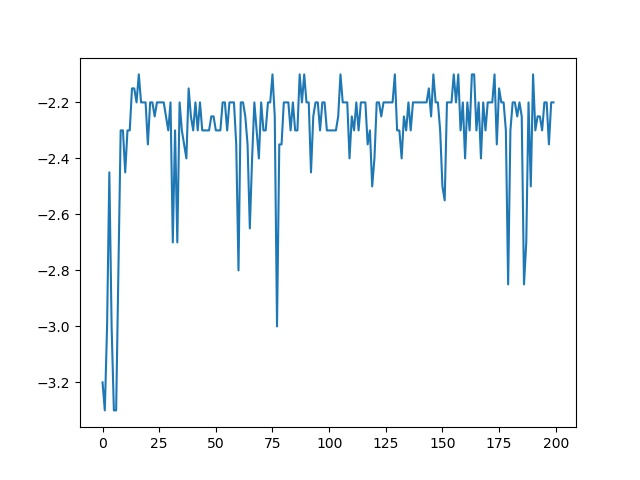
\includegraphics[width=9cm]{3_e_3} 
		\caption{$\epsilon = 0.2$ Asymptote Plot Iterations = 10000} 
		\label{fig:3_2}
		%插入图片的标题,一般放在图片的下方,放在表格的上方
	\end{center}
\end{figure}

\newpage

\subsubsection{Recommended Actions Map}

The score map of the program is shown in figure~\ref{fig:3_3}.


\begin{figure}[htbp] 
	\begin{center}
		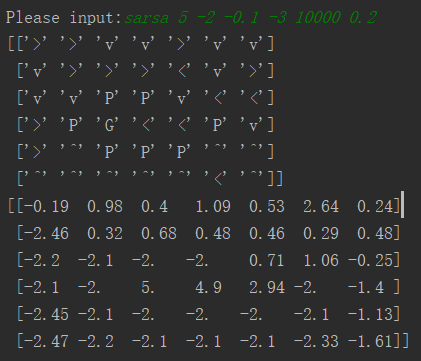
\includegraphics[width=8cm]{3_map} 
		\caption{$\epsilon = 0.2$ Score Map} 
		\label{fig:3_3}
		%插入图片的标题,一般放在图片的下方,放在表格的上方
	\end{center}
\end{figure}


\subsection{$\epsilon$ Exploration}

In this part, the result asymptote plots of the $\epsilon = 0.01$ with iterations 1000 and 10000 are given.

\subsubsection{Iterations = 1000 }

In the figure~\ref{fig:4_1}, the result asymptote plot under the situation $\epsilon = 0.01$ is illustrated. Compared to figure~\ref{fig:1_2} with $\epsilon = 0$, the $\epsilon = 0.01$ illustrated the convergence result with less iterations. 

\begin{figure}[htbp] 
	\begin{center}
		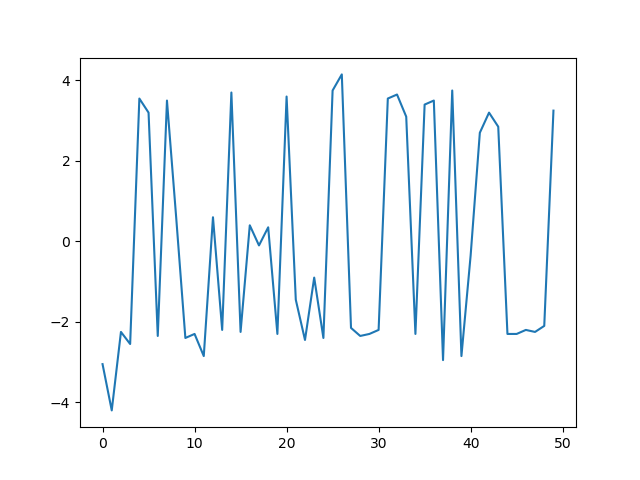
\includegraphics[width=7cm]{4_e_1} 
		\caption{$\epsilon = 0.01$ Asymptote Plot Iterations = 1000} 
		\label{fig:4_1}
		%插入图片的标题,一般放在图片的下方,放在表格的上方
	\end{center}
\end{figure}

\subsubsection{Iterations = 10000}

In the figure~\ref{fig:4_2}, the result asymptote plot under the situation $\epsilon = 0.01$ is illustrated. Compared to figure~\ref{fig:1_2} with $\epsilon = 0$, the $\epsilon = 0.01$ illustrated the convergence result with less iterations. 

\begin{figure}[htbp] 
	\begin{center}
		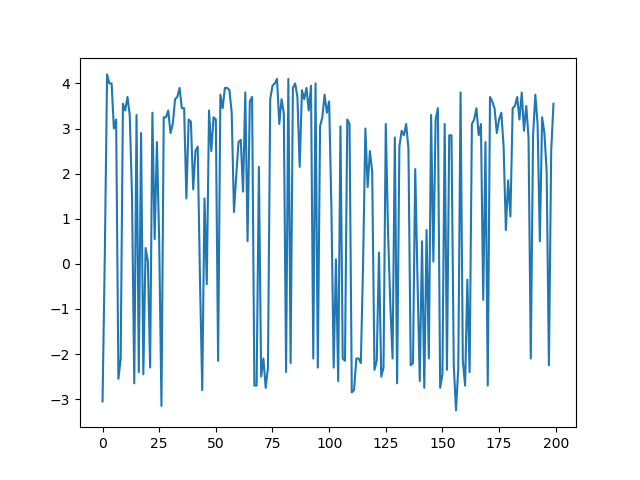
\includegraphics[width=8cm]{4_e_2} 
		\caption{$\epsilon = 0.01$ Asymptote Plot Iterations = 10000} 
		\label{fig:4_2}
		%插入图片的标题,一般放在图片的下方,放在表格的上方
	\end{center}
\end{figure}

\subsubsection{Recommended Actions Map}

The recommended action map of the program is shown in figure~\ref{fig:4_3}.


\begin{figure}[htbp] 
	\begin{center}
		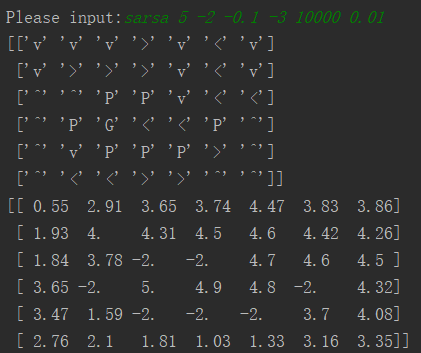
\includegraphics[width=5cm]{4_map} 
		\caption{$\epsilon = 0.01$ Recommended Actions Map} 
		\label{fig:4_3}
		%插入图片的标题,一般放在图片的下方,放在表格的上方
	\end{center}
\end{figure}


\subsection{Parameters Optimization }

\subsubsection{Parameters Not Pointing to Goal}

On the following figures, 2 different model parameters are given: 

\begin{itemize}
\item The result ends in Pit state or give up. 
\item The result ends in Goal state only.
\end{itemize}

In the figure~\ref{fig:5_1}, the recommended action map which leads to pit or give up only is illustrated.

The parameters are on the following: goal reward: -2, pit reward: -2, move action reward: -1, give up reward : -3, $\epsilon = 0.$


\begin{figure}[htbp] 
	\begin{center}
		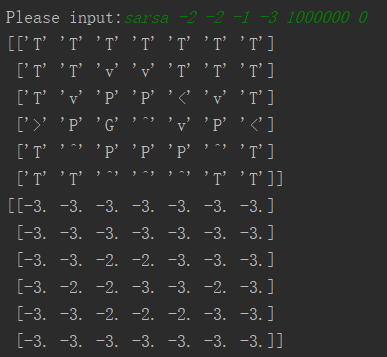
\includegraphics[width=5cm]{5_a_1} 
		\caption{Parameters for Multiple Result} 
		\label{fig:5_1}
		%插入图片的标题,一般放在图片的下方,放在表格的上方
	\end{center}
\end{figure}

In the figure~\ref{fig:5_2}, the recommended action map which leads to goal state only.

The parameters are on the following: goal reward: 5, pit reward: -2, move action reward: -0.01, give up reward : -3, $\epsilon = 0.$


\begin{figure}[htbp] 
	\begin{center}
		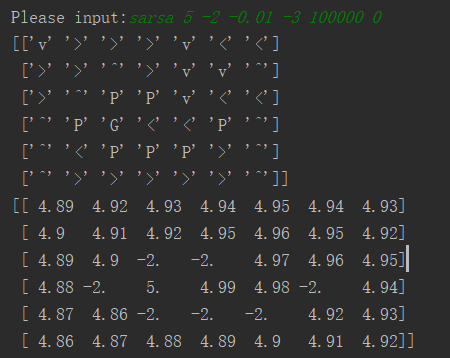
\includegraphics[width=5cm]{5_a_2} 
		\caption{Parameters for Multiple Result} 
		\label{fig:5_2}
		%插入图片的标题,一般放在图片的下方,放在表格的上方
	\end{center}
\end{figure}

\newpage

\subsubsection{Multiple Result}

In the figure~\ref{fig:5_b}, the recommendation action map is given and the parameters are: goal reward: 5, pit reward: -2, move action reward: -1, give up reward : -3, $\epsilon = 0.$


\begin{figure}[htbp] 
	\begin{center}
		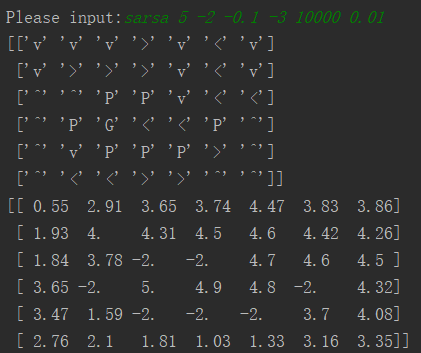
\includegraphics[width=5cm]{4_map} 
		\caption{Parameters for Multiple Result} 
		\label{fig:5_b}
		%插入图片的标题,一般放在图片的下方,放在表格的上方
	\end{center}
\end{figure}



\section{Q functions Initialization (Extra Credit)}

In the program, the Q functions initialization includes the give up reward.
 
The regulation for the Q functions initialization, the value for different 5 states should be 0. In the initialization, the program set the give up reward as -3 directly. 

The initialization is on the following:

$Q(0,0,0,0,0) \rightarrow Q(0,0,0,0,-3)$ 

%-------------------------------------------------------------------------------------------------------





\end{document}
